% Options for packages loaded elsewhere
\PassOptionsToPackage{unicode}{hyperref}
\PassOptionsToPackage{hyphens}{url}
%
\documentclass[
]{book}
\usepackage{amsmath,amssymb}
\usepackage{iftex}
\ifPDFTeX
  \usepackage[T1]{fontenc}
  \usepackage[utf8]{inputenc}
  \usepackage{textcomp} % provide euro and other symbols
\else % if luatex or xetex
  \usepackage{unicode-math} % this also loads fontspec
  \defaultfontfeatures{Scale=MatchLowercase}
  \defaultfontfeatures[\rmfamily]{Ligatures=TeX,Scale=1}
\fi
\usepackage{lmodern}
\ifPDFTeX\else
  % xetex/luatex font selection
\fi
% Use upquote if available, for straight quotes in verbatim environments
\IfFileExists{upquote.sty}{\usepackage{upquote}}{}
\IfFileExists{microtype.sty}{% use microtype if available
  \usepackage[]{microtype}
  \UseMicrotypeSet[protrusion]{basicmath} % disable protrusion for tt fonts
}{}
\makeatletter
\@ifundefined{KOMAClassName}{% if non-KOMA class
  \IfFileExists{parskip.sty}{%
    \usepackage{parskip}
  }{% else
    \setlength{\parindent}{0pt}
    \setlength{\parskip}{6pt plus 2pt minus 1pt}}
}{% if KOMA class
  \KOMAoptions{parskip=half}}
\makeatother
\usepackage{xcolor}
\usepackage{longtable,booktabs,array}
\usepackage{calc} % for calculating minipage widths
% Correct order of tables after \paragraph or \subparagraph
\usepackage{etoolbox}
\makeatletter
\patchcmd\longtable{\par}{\if@noskipsec\mbox{}\fi\par}{}{}
\makeatother
% Allow footnotes in longtable head/foot
\IfFileExists{footnotehyper.sty}{\usepackage{footnotehyper}}{\usepackage{footnote}}
\makesavenoteenv{longtable}
\usepackage{graphicx}
\makeatletter
\def\maxwidth{\ifdim\Gin@nat@width>\linewidth\linewidth\else\Gin@nat@width\fi}
\def\maxheight{\ifdim\Gin@nat@height>\textheight\textheight\else\Gin@nat@height\fi}
\makeatother
% Scale images if necessary, so that they will not overflow the page
% margins by default, and it is still possible to overwrite the defaults
% using explicit options in \includegraphics[width, height, ...]{}
\setkeys{Gin}{width=\maxwidth,height=\maxheight,keepaspectratio}
% Set default figure placement to htbp
\makeatletter
\def\fps@figure{htbp}
\makeatother
\setlength{\emergencystretch}{3em} % prevent overfull lines
\providecommand{\tightlist}{%
  \setlength{\itemsep}{0pt}\setlength{\parskip}{0pt}}
\setcounter{secnumdepth}{5}
\usepackage{booktabs}
\ifLuaTeX
  \usepackage{selnolig}  % disable illegal ligatures
\fi
\usepackage[]{natbib}
\bibliographystyle{apalike}
\usepackage{bookmark}
\IfFileExists{xurl.sty}{\usepackage{xurl}}{} % add URL line breaks if available
\urlstyle{same}
\hypersetup{
  pdftitle={A protocol for sequencing and analysing 16S-ITS-23S amplicons using Oxford Nanopore's Native Barcoding kit to profile prokaryotes on species-level in a mixed community {[}Under development{]}},
  pdfauthor={Christian Krohn, PhD, RMIT University},
  hidelinks,
  pdfcreator={LaTeX via pandoc}}

\title{A protocol for sequencing and analysing 16S-ITS-23S amplicons using Oxford Nanopore's Native Barcoding kit to profile prokaryotes on species-level in a mixed community {[}Under development{]}}
\author{\href{https://www.rmit.edu.au/contact/staff-contacts/academic-staff/k/krohn---christian}{Christian Krohn, PhD, RMIT University}}
\date{2024-06-17}

\begin{document}
\maketitle

{
\setcounter{tocdepth}{1}
\tableofcontents
}
\chapter{About this GitBook}\label{about}

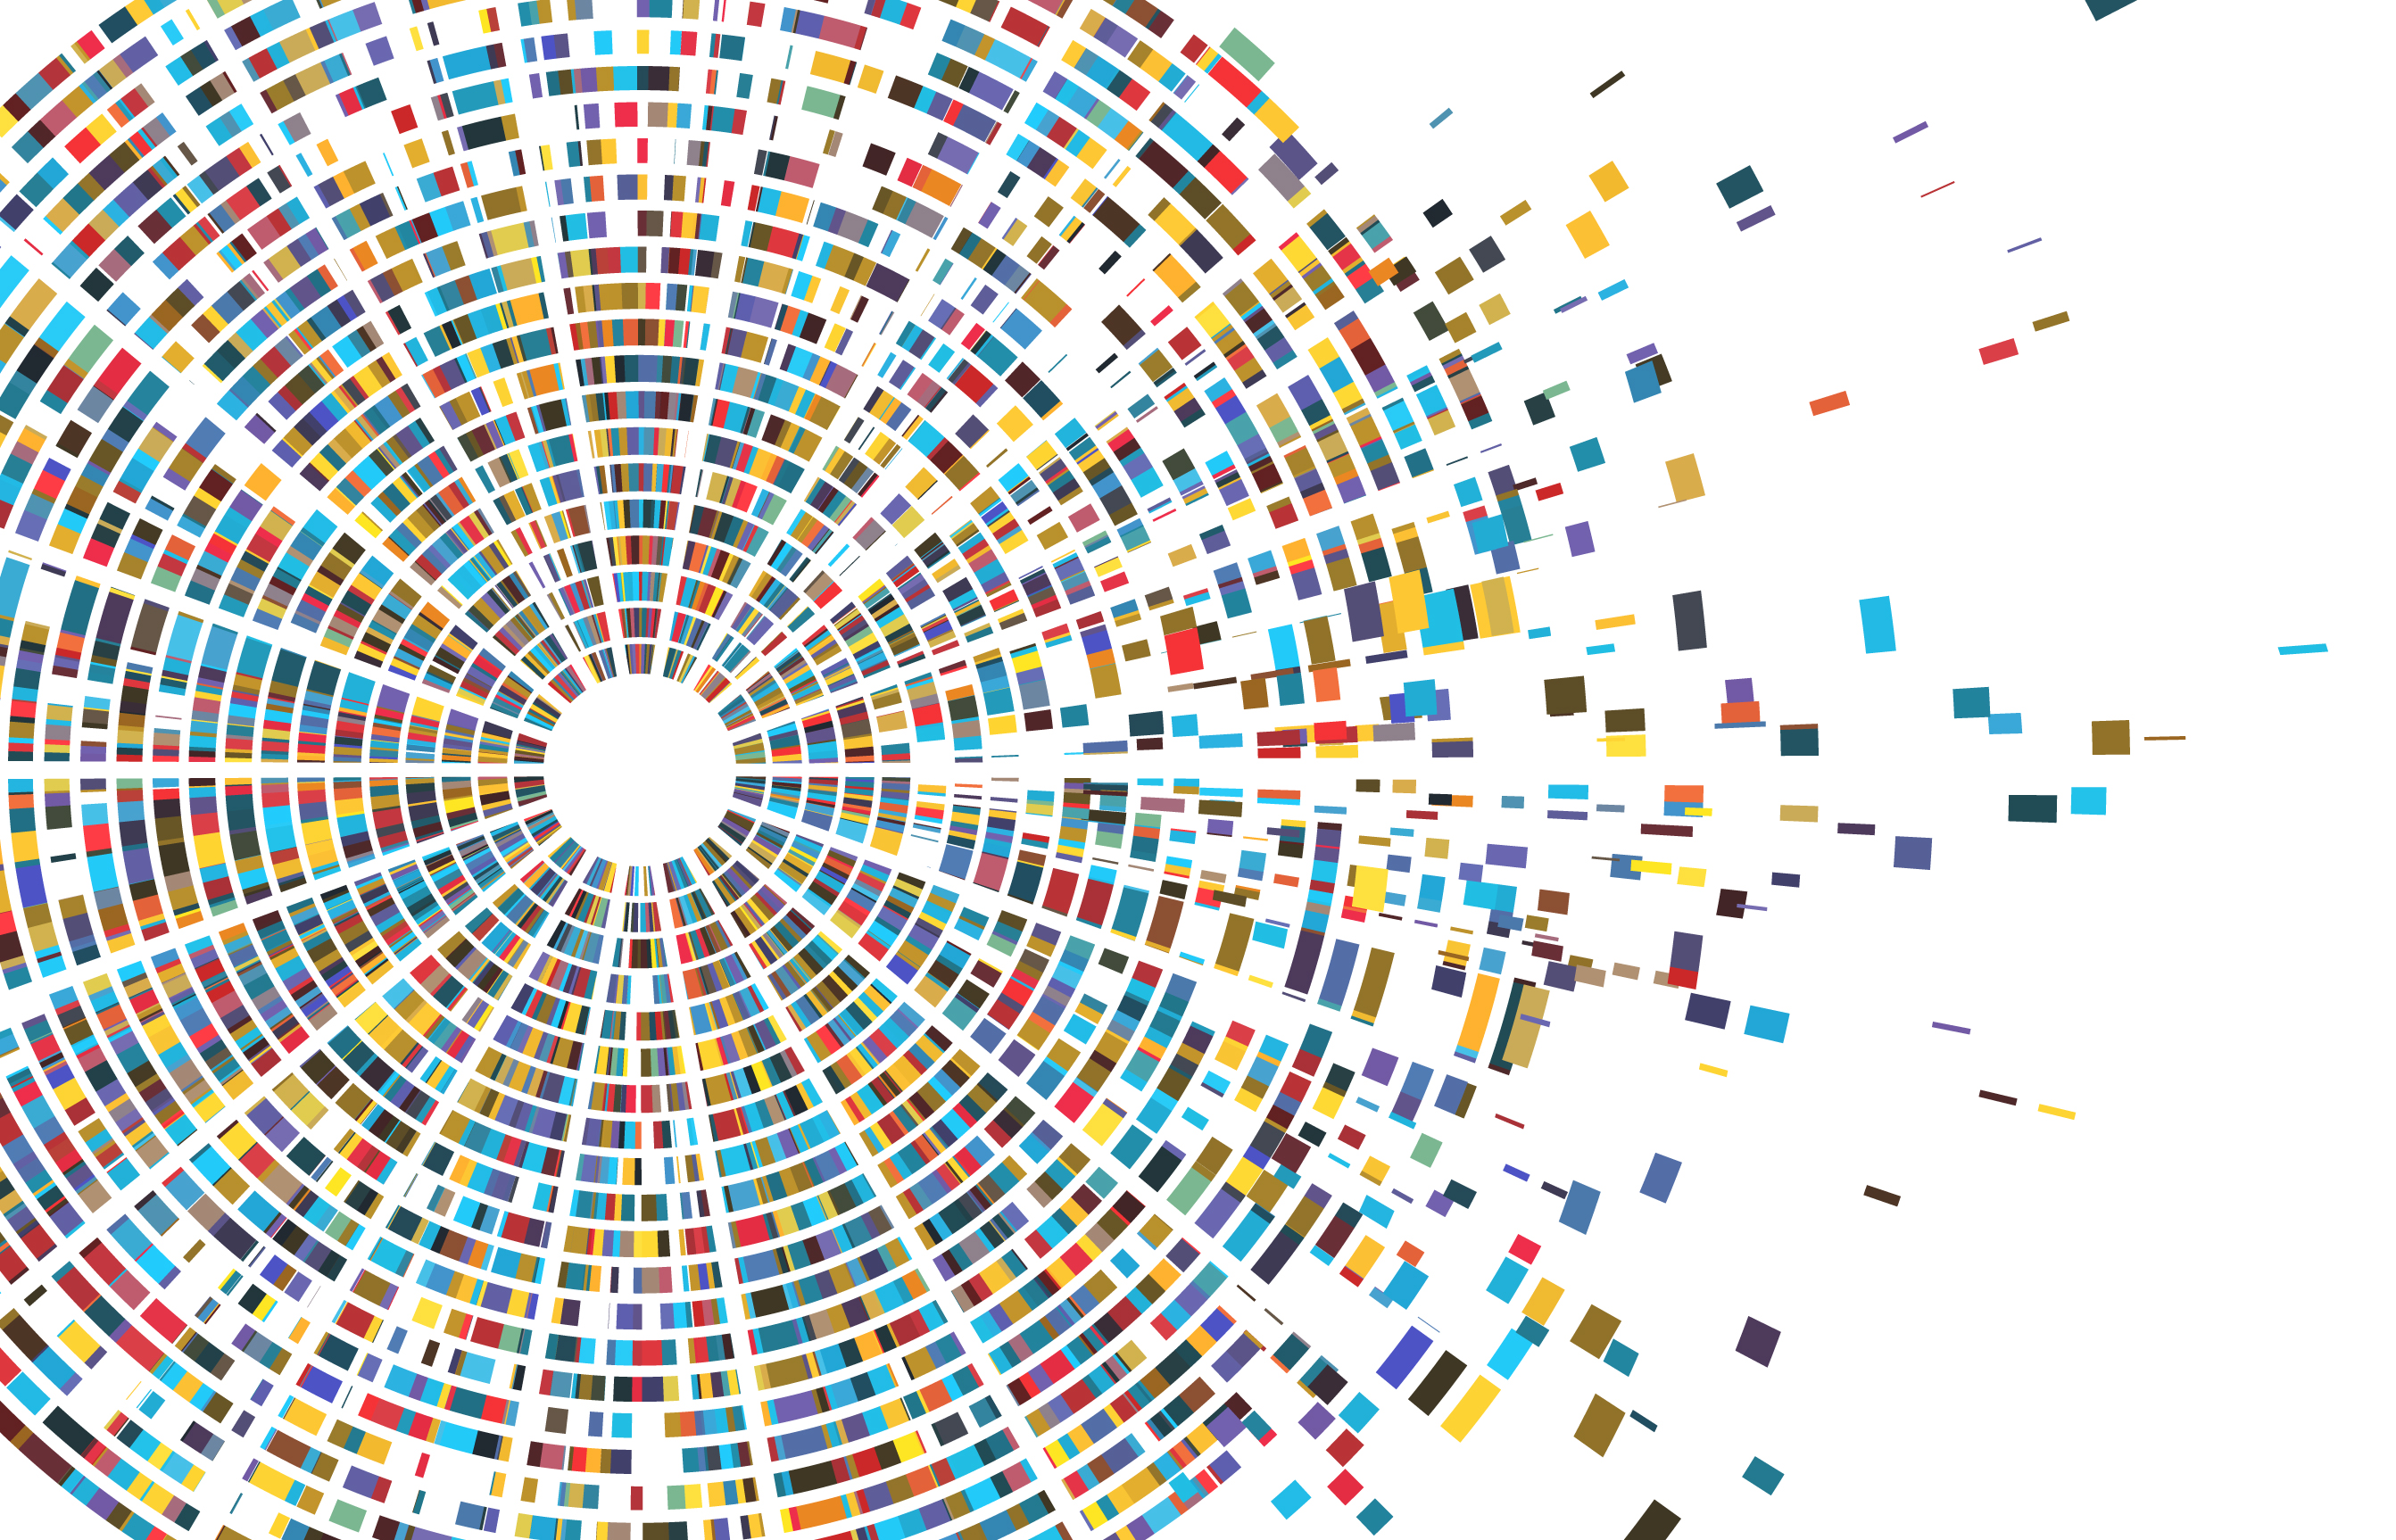
\includegraphics[width=5.20833in,height=\textheight]{./img/vectorstock_23650232.jpg}

This GitBook is under development (2024).

This GitBook provides a basic step-by-step protocol for students who want to get started with sequencing multiple samples of high quality, full-length microbial amplicons with an Oxford Nanopore instrument, and then process and visualise the data using various packages in R.

This protocol reflects the experiences we had in the lab and may help to get you started on your own journey of discovery. One of the biggest hurdles for students that embark on sequencing environmental DNA for the first time, is the effort required to learn new technologies, various coding languages, file types and formats, packages or platforms that are involved (think Unix, Linux, Slurm, Qiime, R, RMarkdown, python, conda, ggplot, docker, GitHub, data instances\ldots) before they even can start looking at exploring the data for biological meaning and producing publishable output. Hence, this protocol aims at lowering your `activation' energy by providing some guidance for each step from DNA extraction, to amplification, library preparation, sequencing, data processing and finally some basic visualisations in R.

This protocol uses the DNeasy Powersoil Pro Kit (Qiagen, Hilden, Germany) to extract DNA from wastewater sludge, as well as the Native Barcoding Kit (SQK-NBD114.96) with a R10.4.1 flowcell (FLO-MIN114) to sequence long (\textasciitilde4-4.4 kb) amplicons from environmental DNA. The primer used was developed by \citep{Martijn2019}. Initial costs to purchase all consumables will be \textasciitilde AUD\$7,700.

Check out our workflows for short-read 16S sequencing at \url{https://chrismitbiz.github.io/ABlab-workflows} if you want to get started with Miseq 16S sequencing instead.

If you are interested in sequencing the living biomass via PMA treatment in combination with short-read 16S sequencing, check out our recent paper \href{https://doi.org/10.1016/j.watres.2024.121354}{Dead in the water -- Role of relic DNA and primer choice for targeted sequencing surveys of anaerobic sewage sludge intended for biological monitoring} \citep{Krohn2024}

\textbf{Get in touch}

We work at the Andy Ball lab, RMIT University, Bundoora, Melbourne and are part of the Industry-led \href{https://www.transformingbiosolids.org.au}{Biosolids Training Centre}. Email me or comment on the discussion section of the \href{https://github.com/chrismitbiz/ABlab-workflows/discussions/}{GitHub repository} for this GitBook. You will need to get a GitHub account to join the discussion. Its free.

More about me and my PhD research can be found here: \url{https://clean-dirt-digests.netlify.app}.\\
Follow me on \href{https://twitter.com/CleanDirtChris}{Twitter} or \href{https://www.linkedin.com/in/christian-krohn-54904855}{LinkedIn}.

~

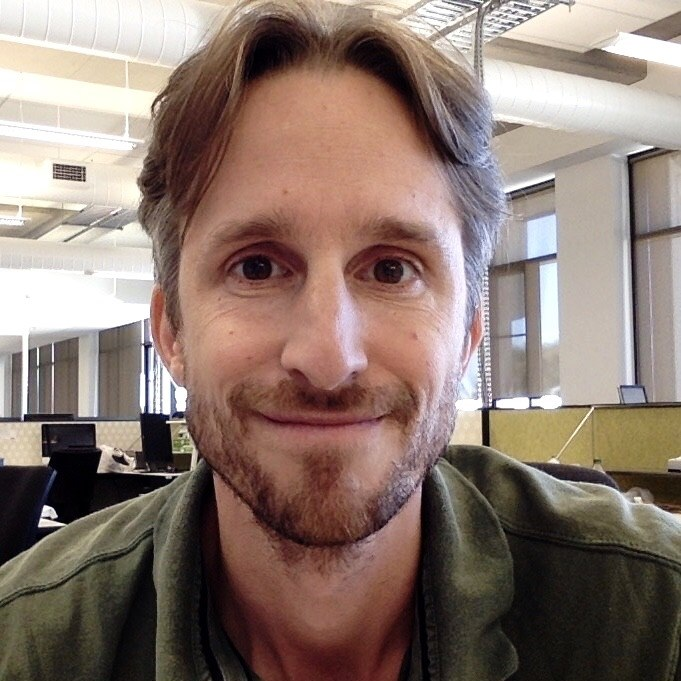
\includegraphics[width=1.5625in,height=\textheight]{./img/avatar.jpg}

Bio:\\
Dr Chris Krohn is an early career researcher whose interests could be summed up with: ``Environmental sequencing, microbial ecology, chlorinated pollutants, organic matter, wastewater, anaerobic digestion, and how everything connects''.

In 2021 I joined the ARC Biosolids Training Centre at RMIT (www.transformingbiosolids.org.au), where we help water utilities to improve circular resource management by getting more renewable biogas and carbon/fertiliser values out of our municipal biosolids (essentially our poo). In project 1C of the Centre I develop metagenomic (DNA-based) methods to monitor the microbiome of anaerobic digestion, an important microbial treatment process for wastewater. I believe DNA-based diagnoses of wastewater sludges will help the water/biosolids sector improve resource recoveries and risk management.

Before that, after a career in one of the most fast-cycled and short-sighted manufacturing industries that took me from Germany to Vietnam and Hong Kong/Shenzhen, I decided to hit the switch and start thinking long-term and circular. Ten back-to-uni years later, in 2021 I finished a PhD in Soil Science at La Trobe Uni where I sequenced soil DNA and explored if and how soil biology was involved in the degradation of extremely persistent legacy pesticides that contaminate agricultural surface soils since several decades.\\

This work is licensed under a Creative Commons Attribution 4.0 International License.

\chapter{Prerequisites and consumables}\label{prerequisites}

\section{Prerequisites}\label{prerequisites-1}

\begin{itemize}
\tightlist
\item
  Experience with basic molecular lab technique and DNA quality control (use of laminar flow hood, pipetting micro volumes, handling and preserving small volume reagents, sterilisation of consumables, doing gel electrophoresis)
\item
  Experience with loading Nanopore flowcells (for example by doing a test run with Lambda DNA using the \href{https://store.nanoporetech.com/control-expansion.html}{Control Expansion Kit})\\
\item
  Confident with R, R Studio and package environment managers such as Conda and Docker. Knowledge in shell scripting and Linux syntax.
\end{itemize}

\section{DNA extraction kit}\label{dna-extraction-kit}

We commonly extract DNA from soils or from wastewater sludges using the DNeasy Powersoil Pro Kit (Qiagen) for both, soil and sludge. It resulted in high quality DNA, suitable for library preparation and sequencing. Extraction with this kit includes a bead beating step to release DNA from cells out of difficult matrices such as soils and sludge (biofilms) or similar. The sheared DNA will be fragmented with a N50 of \textasciitilde7 kb in some cases \citep{Jensen2024}. Shearing of DNA may be minimised by reducing/optimising bead-beating duration and speed. Other commonly used and commercially available kits for DNA extraction are available \citep{Jensen2024, Gand2023}.

\begin{figure}
\centering
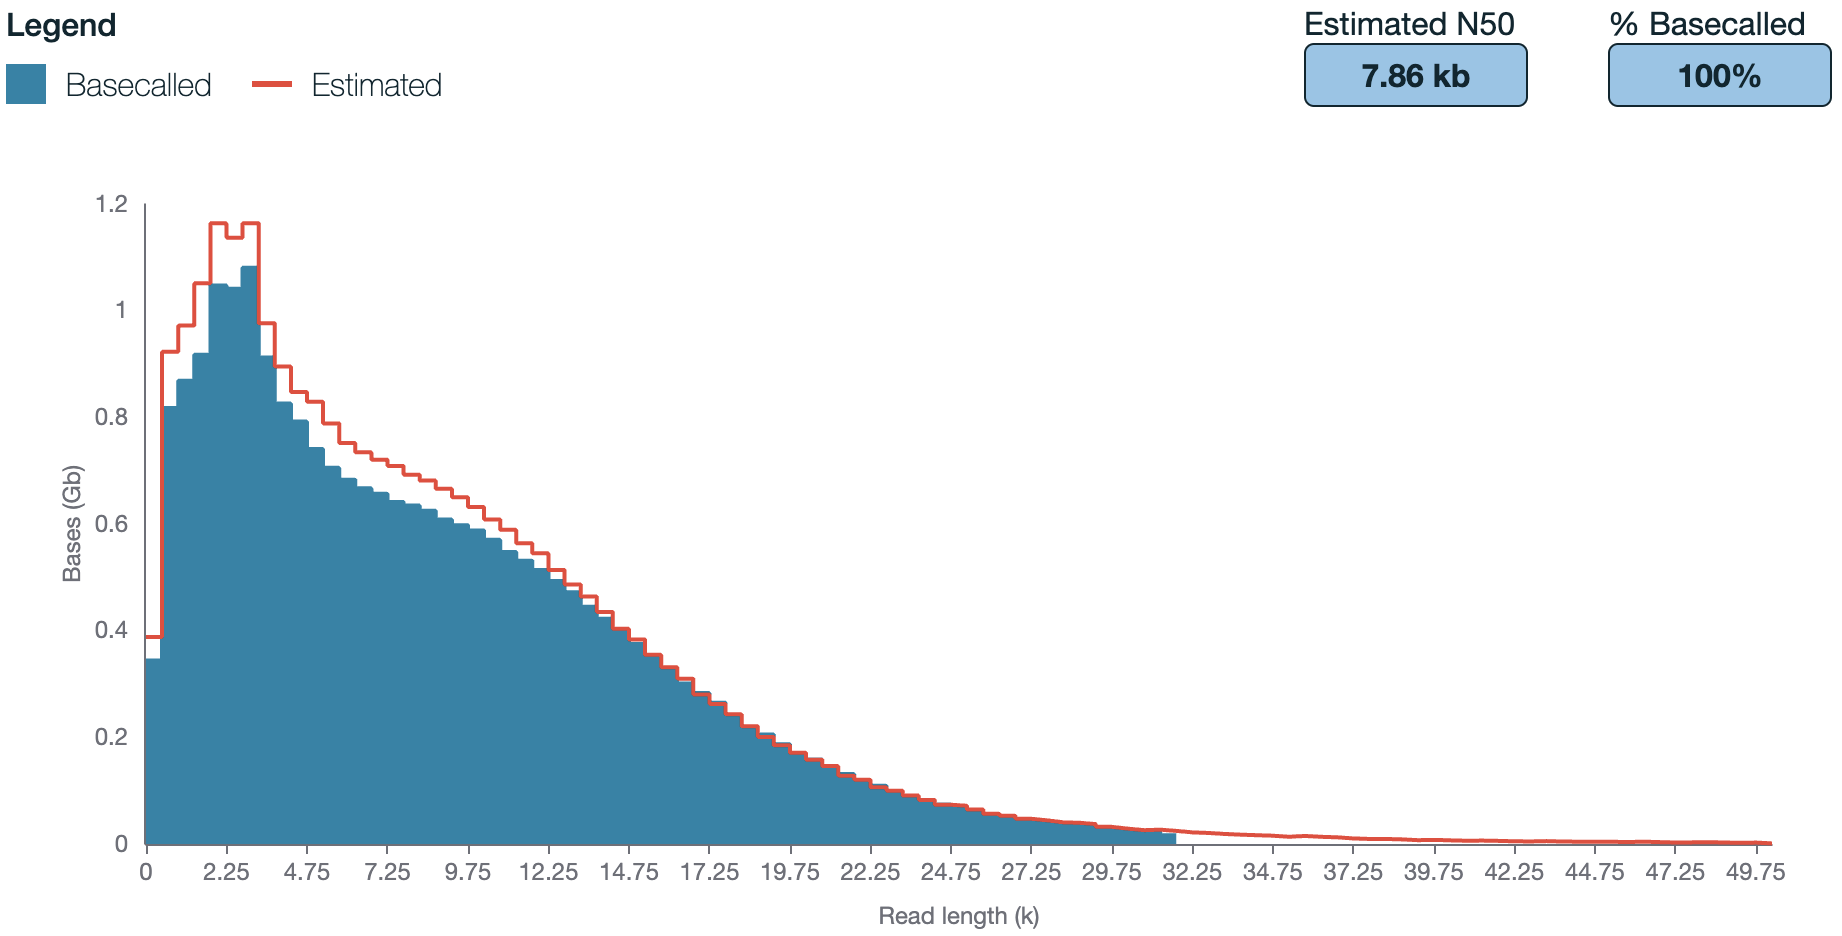
\includegraphics[width=6.25in,height=\textheight]{./img/readsize.png}
\caption{``Example of read size distribution of sludge DNA extracted with the DNeasy Powersoil Pro Kit in our lab''}
\end{figure}

\section{Consumables}\label{consumables}

\begin{itemize}
\tightlist
\item
  Native Barcoding Kit (Oxford Nanopore, SQK-NBD114.96)\\
\item
  R10.4.1 flowcell (Oxford Nanopore, FLO-MIN114)
\item
  NEBNext Quick Ligation Module (E6056, New England Biolab)
\item
  NEBNext Ultra II End repair/dA-tailing Module (E7546S, New England Biolab)
\item
  Blunt/TA Ligase Master Mix (M0367, New England Biolab)
\item
  10 mM dNTPs (N0447S, New England Biolab)
\item
  Q5 Hot Start High-Fidelity DNA Polymerase (M0493, New England Biolab)
\item
  DNeasy Powersoil Pro Kit (\#47016, Qiagen)
\item
  Qubit 1X dsDNA BR Assay Kit (Q33266, Thermo Fisher)
\item
  Eppendorf LoBind tubes (Eppendorf)
\item
  twin.tec® PCR plate 96 LoBind, semi skirted (0030129504, Eppendorf)
\item
  JetSeq Clean Magnetic beads (MER-BIO-68031, Millenium Science) - to clean up PCR products
\item
  10 µM Forward Primer A519F (CAGCMGCCGCGGTAA) \citep{Martijn2019}
\item
  10 µM Reverse Primer U2428R (CCRAMCTGTCTCACGACG) \citep{Martijn2019}
\item
  Nuclease-free water
\item
  10 mM Tris-HCl pH 8.0 with 50 mM NaCl (UltraPure™ 1M Tris-HCI, pH 8.0 \#15568025 \& NaCl (5 M), RNase-free \#AM9760G, Thermo Fisher)
\item
  Bovine Serum Albumin (BSA) (50 mg/ml) (AM2616, InvitrogenTM UltraPure)
\item
  HyperLadder 1kb (BIO-33025, Bioline, Millenium Science)
\item
  80\% ethanol, freshly prepared in nuclease-free water
\end{itemize}

\section{Protocols}\label{protocols}

\begin{itemize}
\tightlist
\item
  A protocol for PCR amplification and clean-up (included in this Gitbook).
\item
  `Ligation sequencing amplicons - Native Barcoding Kit 96 V14' available on nanoporetech.com - Checklist and full protocol.
\item
  Prepare spreadsheets to normalise DNA into 96-well plates to avoid pipetting errors.
\end{itemize}

\section{Equipment}\label{equipment}

\begin{itemize}
\tightlist
\item
  Nanopore sequencer. This protocol is based on the MinION Mk1C but is not limited to this model.
\item
  Nanodrop spectrophotometer to check DNA quality.
\item
  Qubit fluorometer (Thermo Fisher).
\item
  PCR thermal cycler.
\item
  Gel electrophoresis equipment.
\item
  Vortex. We use the Vortex-Genie 2, including the 24 x 2 ml tube adapter for bead beating.
\end{itemize}

\section{Computational resources and database}\label{computational-resources-and-database}

\begin{itemize}
\tightlist
\item
  An instance or computer with ≥ 2 TB storage, ≥ 64 GB RAM and ≥ 32 CPUs
\item
  16S-ITS-23S Database. To be confirmed.
\end{itemize}

\chapter{Protocol}\label{protocol}

\section{DNA extraction}\label{dna-extraction}

\subsection{Checklist}\label{checklist}

\begin{itemize}
\tightlist
\item
  Extraction kit - \href{https://www.qiagen.com/au/resources/resourcedetail?id=9bb59b74-e493-4aeb-b6c1-f660852e8d97&lang=en}{DNeasy Powersoil Pro, Qiagen, Hilden, Germany}
\item
  Alternatively the high throughput version of the kit used with the QIAcube \href{https://rmiteduau-my.sharepoint.com/personal/christian_krohn_rmit_edu_au/Documents/Experiments/2025_ETPSequencingProject/_\%09https:/www.qiagen.com/au/products/discovery-and-translational-research/dna-rna-purification/dna-purification/microbial-dna/dneasy-96-powersoil-pro-qiacube-ht-kit}{DNeasy 96 PowerSoil Pro QIAcube HT Kit}
\item
  Vortex with 24 x 1.5 mL tube adapter (e.g.~Vortex Genie 2 + adapter). Alternatively, a PowerLyzer Homogenizer.
\item
  NanoDrop spectrophotometer to assess DNA quality.
\item
  Qubit fluorometer for accurately measure DNA concentrations.
\end{itemize}

\subsection{Process}\label{process}

\begin{itemize}
\tightlist
\item
  Follow the extraction kit's protocol with 15 mins bead beating with Genie vortex and 24-tube adapter. Reduce this to 10 mins if less than 24 samples are extracted or if shearing of DNA should be minimised.
\item
  Measure DNA quality using DNA extract (1 µL) using a Nanodrop spectrophotometer
\item
  Measure DNA concentration using a Qubit fluorometer.
\item
  Into a 96-well plate, normalise extracted DNA to required PCR concentrations. For example, if 10 ng template is required for PCR, normalise DNA to 5 ng/µL and use 2 µL.\\
\item
  Store DNA at 4˚C until library preparation - no more than 1 week.
\item
  Store DNA at -20˚C if sequencing is more than 1 week away.
\end{itemize}

\section{DNA library preparation and PCR}\label{dna-library-preparation-and-pcr}

\subsection{DNA Library preparation including PCR, multiplexing and pooling of samples.}\label{dna-library-preparation-including-pcr-multiplexing-and-pooling-of-samples.}

\subsection{Checklist}\label{checklist-1}

\begin{itemize}
\tightlist
\item
  10 mM dNTPs (N0447S, New England Biolab)
\item
  Q5 Hot Start High-Fidelity DNA Polymerase (M0493, New England Biolab)
\item
  10 µM Forward Primer A519F (CAGCMGCCGCGGTAA) \citep{Martijn2019}
\item
  10 µM Reverse Primer U2428R (CCRAMCTGTCTCACGACG) \citep{Martijn2019}
\item
  JetSeq Clean Magnetic beads - or equivalent (MER-BIO-68031, Millenium Science) - to clean up PCR products\\
\item
  twin.tec® PCR plate 96 LoBind, semi skirted (0030129504, Eppendorf)\\
\item
  Nuclease-free water
\item
  10 mM Tris-HCl pH 8.0 with 50 mM NaCl (UltraPure™ 1M Tris-HCI, pH 8.0 \#15568025 \& NaCl (5 M), RNase-free \#AM9760G, Thermo Fisher)\\
\item
  HyperLadder 1kb (BIO-33025, Bioline, Millenium Science)
\item
  80\% ethanol, freshly prepared in nuclease-free water
\item
  Qubit 1X dsDNA BR Assay Kit (Q33266, Thermo Fisher)
\end{itemize}

\textbf{Notes}

\begin{itemize}
\tightlist
\item
  Do not vortex tubes during library preparation and use wide-bore tips to prevent DNA fragmentation. Fragmentation of amplicons may lead to incomplete reads.\\
\item
  The primer amplifies the whole rrn operon.
\end{itemize}

Benefits of targeting the whole rrn operon:

\begin{itemize}
\tightlist
\item
  Superior species-level resolution and accuracy \citep{Cusco2018, Srinivas2024}.\\
\item
  Covers Bacteria and Archaea.
\end{itemize}

Risks of targeting the whole rrn operon:

\begin{itemize}
\tightlist
\item
  Not as representative of true abundances as full-length 16S amplicons.\\
\item
  Species with unlinked 16S and 23S rrn DNA will be missed with this approach (for example \textless{} 9\% of rRNA genes in wastewater sludge \citep{Brewer2020}).
\end{itemize}

\subsection{PCR}\label{pcr}

Time required \textasciitilde4 hrs incl.~2hrs, 40mins PCR.

\begin{itemize}
\tightlist
\item
  Prepare a mastermix for required number of 50 µl reactions.
\item
  Add 3 µl of eDNA (5ng /µl) into a 96-well plate (e.g.~Eppendorf twin.tec® PCR plate 96 LoBind, semi-skirted) using a multichannel pipette.\\
\item
  Add 47 µl of mastermix using a multichannel pipette and carefully pipette up and down 10 x
\item
  Run thermocycler.
\item
  Verify amplification length via 1\% agarose gel electrophoresis @ 100V for 30 min including a 1 kb ladder (Fig. 2).
\item
  Store at 4˚C overnight if needed.
\end{itemize}

\textbf{Important}:

\begin{itemize}
\tightlist
\item
  Use hot start polymerase for ease of use, with high fidelity/accuracy and one that is suitable for long amplicons. For example, Q5 High- Fidelity DNA Polymerase kit (New England Biolabs) with GC enhancer \citep{Martijn2019}.\\
\item
  ≤ 200 fmol is required per sample for the Native Barcoding Kit from ONP. Based on 4.25 kb (4-4.5kb), the final DNA concentration after cleaning up PCR products should be no less than 48 ng/µL (at 11.5 µl input volume) - giving 552 ng of 4.25kb amplicons.\\
\item
  It may require two--three PCR reactions to achieve the required DNA amount (200 fmol); e.g.~pool 2--3 x 50µl PCR products, clean combined and elude in 32.5 µl Tris.
\end{itemize}

\begin{verbatim}
## -- Attaching core tidyverse packages ------------------------ tidyverse 2.0.0 --
## v dplyr     1.1.4     v readr     2.1.5
## v forcats   1.0.0     v stringr   1.5.1
## v ggplot2   3.5.1     v tibble    3.2.1
## v lubridate 1.9.3     v tidyr     1.3.1
## v purrr     1.0.2     
## -- Conflicts ------------------------------------------ tidyverse_conflicts() --
## x dplyr::filter() masks stats::filter()
## x dplyr::lag()    masks stats::lag()
## i Use the conflicted package (<http://conflicted.r-lib.org/>) to force all conflicts to become errors
\end{verbatim}

\begin{table}

\caption{\label{tab:table}List of components for each reaction (each tube) for PCR. See https://www.neb.com/en-au/protocols/2012/08/30/pcr-using-q5-hot-start-high-fidelity-dna-polymerase-m0493 for details.  }
\centering
\begin{tabular}[t]{lll}
\toprule
Component & 50 µl reaction & Final concentration\\
\midrule
5X Q5 Reaction Buffer - M0493S NEB & 10 µL & 1X\\
10 mM dNTPs N0447S & 1 µL & 200 µM\\
10 µM Forward Primer & 2.5 µL & 0.5 µM\\
10 µM Reverse Primer & 2.5 µl & 0.5 µM\\
Template DNA - 15 ng & 3 µL (5 ng/µL) & < 1,000 ng\\
\addlinespace
Q5 Hot StartÊHigh-Fidelity DNA Polymerase -M0493S NEB & 1.0 µL & 0.04 U/µL\\
5X Q5 High GC Enhancer M0493S NEB & 10 µL & (1X)\\
Nuclease-Free Water & to 50 µL & \\
\bottomrule
\end{tabular}
\end{table}

  \bibliography{book.bib,packages.bib}

\end{document}
